% Q4: C-Core Electromagnet — Physical drawing with air gap and coil
% Uses TikZ (not CircuiTikZ) for geometric/physical drawing
\documentclass[border=10pt]{standalone}
\usepackage{tikz}
\usepackage{amsmath}
\renewcommand{\familydefault}{\sfdefault}

\begin{document}
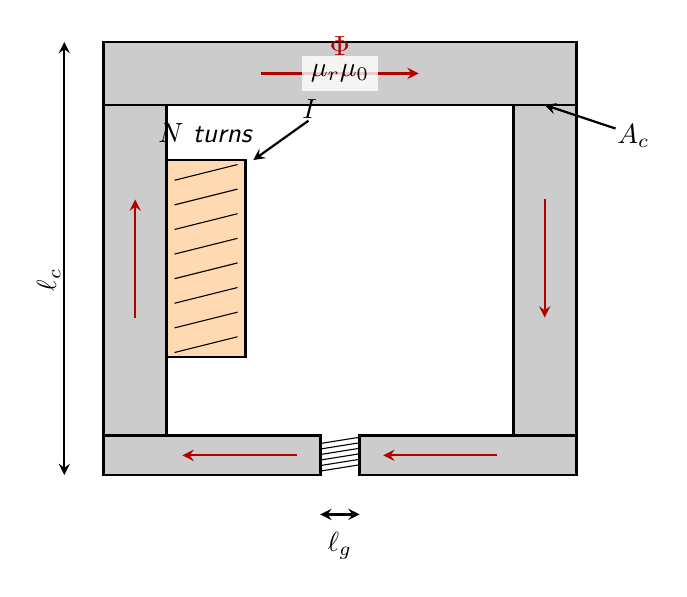
\begin{tikzpicture}[
    every node/.style={font=\sffamily},
    >=stealth
]

% Parameters
\def\outerW{6.0}
\def\outerH{5.5}
\def\coreW{0.8}
\def\gapW{0.5}

% === Core pieces (C-shape) ===
\pgfmathsetmacro{\halfgap}{\gapW/2}
\pgfmathsetmacro{\halfW}{\outerW/2}
\pgfmathsetmacro{\botH}{0.5}

% Top horizontal bar
\fill[gray!40, draw=black, line width=1pt]
    (0,{\outerH-\coreW}) rectangle (\outerW,\outerH);

% Left vertical leg
\fill[gray!40, draw=black, line width=1pt]
    (0,\gapW) rectangle (\coreW,{\outerH-\coreW});

% Right vertical leg
\fill[gray!40, draw=black, line width=1pt]
    ({\outerW-\coreW},\gapW) rectangle (\outerW,{\outerH-\coreW});

% Bottom bar — left half (up to gap)
\fill[gray!40, draw=black, line width=1pt]
    (0,0) rectangle ({\halfW-\halfgap},\botH);

% Bottom bar — right half (after gap)
\fill[gray!40, draw=black, line width=1pt]
    ({\halfW+\halfgap},0) rectangle (\outerW,\botH);

% === Air gap hatching ===
\foreach \y in {0.05, 0.12, 0.19, 0.26, 0.33, 0.40} {
    \draw[thin] ({\halfW-\halfgap},\y) -- ({\halfW+\halfgap},{\y+0.08});
}

% === Coil on left leg ===
\fill[orange!30, draw=black, line width=0.8pt]
    (\coreW,1.5) rectangle ({\coreW+1.0},4.0);

% Diagonal winding lines inside coil
\foreach \i in {0,...,7} {
    \pgfmathsetmacro{\yline}{1.5 + (\i+0.5)*2.5/8}
    \draw[thin] ({\coreW+0.1},{\yline-0.1}) -- ({\coreW+0.9},{\yline+0.1});
}

% Coil label
\node[above] at ({\coreW+0.5},4.1) {\textit{$N$ turns}};

% Current arrow
\draw[->, line width=0.8pt]
    ({\coreW+1.8},4.5) -- ({\coreW+1.1},4.0);
\node[above right] at ({\coreW+1.6},4.4) {$I$};

% === Flux arrows (clockwise) ===
% Top bar: left to right
\draw[->, red!70!black, thick] (2.0,{\outerH-\coreW/2}) -- (4.0,{\outerH-\coreW/2});
\node[red!70!black, above] at (3.0,{\outerH-\coreW/2+0.1}) {$\Phi$};

% Right leg: top to bottom
\draw[->, red!70!black, thick] ({\outerW-\coreW/2},3.5) -- ({\outerW-\coreW/2},2.0);

% Bottom bar right side: right to left
\draw[->, red!70!black, thick] ({\outerW-\coreW-0.2},{\botH/2}) -- ({\halfW+\halfgap+0.3},{\botH/2});

% Bottom bar left side: right to left (through gap)
\draw[->, red!70!black, thick] ({\halfW-\halfgap-0.3},{\botH/2}) -- (1.0,{\botH/2});

% Left leg: bottom to top
\draw[->, red!70!black, thick] ({\coreW/2},2.0) -- ({\coreW/2},3.5);

% === Dimension labels ===
% Core height (ℓ_c)
\draw[<->, line width=0.8pt] (-0.5,0) -- (-0.5,\outerH);
\node[left, rotate=90] at (-0.7,{\outerH/2}) {$\ell_c$};

% Air gap length (ℓ_g)
\draw[<->, line width=0.8pt] ({\halfW-\halfgap},-0.5) -- ({\halfW+\halfgap},-0.5);
\node[below] at (\halfW,-0.6) {$\ell_g$};

% Cross-section label (A_c)
\draw[->, line width=0.8pt]
    ({\outerW+0.5},{\outerH-\coreW-0.3}) -- ({\outerW-\coreW/2},{\outerH-\coreW});
\node[right] at ({\outerW+0.4},{\outerH-\coreW-0.4}) {$A_c$};

% Permeability label on core
\node[fill=white, fill opacity=0.8, text opacity=1]
    at ({\outerW/2},{\outerH-\coreW/2}) {$\mu_r \mu_0$};

\end{tikzpicture}
\end{document}
